\documentclass[12pt]{article}
\usepackage[utf8]{inputenc}
\usepackage[a4paper, margin=1in]{geometry}
\usepackage{graphicx}
\usepackage{amsmath}
\usepackage{fancyhdr}
\usepackage{color}
\usepackage{titlesec}
\usepackage{tikz}
\usepackage{wrapfig}  
\usepackage[a4paper,top=2.8cm,bottom=0.8cm,left=2.5cm,right=2.5cm]{geometry}
\usepackage{mathptmx} 
\usepackage{titlesec}
\usepackage{xcolor}
\usepackage{enumitem}
\usepackage{setspace}
\usepackage{titling}
\usepackage{lipsum}
\usepackage{float}
\usepackage{caption}
\usepackage{subcaption}
\pagestyle{empty}
\setlength{\parindent}{0pt}
\setlength{\parskip}{0.8em}
\setstretch{1.1}
\definecolor{chapterblue}{RGB}{0,174,239} 
\definecolor{darkskyblue}{rgb}{0.0, 0.5, 1.0}
\definecolor{skyblue}{RGB}{135, 206, 235}
\usepackage{newtxtext,newtxmath}
\titleformat{\section}
  {\fontsize{67}{48}\selectfont\bfseries\color{chapterblue}}{\thesection}{1em}{}
% Title format
\titleformat{\section}
  {\normalfont\Large\bfseries\color{chapterblue}}{\thesection}{1em}{}
% Header/Footer settings
\pagestyle{fancy}
\cfoot{2019-2}
\renewcommand{\headrulewidth}{0pt}
\renewcommand{\footrulewidth}{0pt}
\begin{document}
\begin{enumerate}
\pagestyle{empty} % Start with empty page style
\thispagestyle{fancy} % Apply fancy style only to the first page 
\renewcommand{\headrulewidth}{0pt} % Remove header rule
\fancyhead[L]{% Left header
        
\includegraphics[width=7cm, height=1.5cm]{img3.png} 
        }
\fancyhead[R]{% Right header
    Name: S.Rithrishareddy \\
    Batch: COMETFWC028\\
    Date: 18 may 2025
}
\begin{center}
   \vspace{8em} \includegraphics[width=80]{scanner.png} % Replace with your QR image
\end{center}
\begin{center}
\hfill
\vspace{-4em}
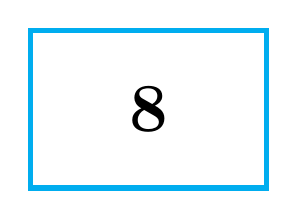
\begin{tikzpicture}
    \vspace{6em}\draw[line width=2pt, draw=cyan ] (0,0) rectangle (3,2);
     \node at (1.5,1) {\textcolor{black}{\fontsize{60pt}{60pt}\selectfont \textbf{8}}};
\end{tikzpicture}
 \vspace{-0.5em}
\begin{center}
\vspace{-2em}
    {\textcolor{chapterblue}{
        \textbf{
               {\fontsize{30}{40}\selectfont I}{\fontsize{20}{34}\selectfont NTRODUCTION TO }\\         
           \vspace{1em} {\fontsize{30}{46}\selectfont T}{\fontsize{20}{34}\selectfont RIGNOMETRY}
             % Pull the line up to sit just under the text
                       }
  }
\end{center}
\vspace{-2em} % adjust vertical spacing between title and line
\noindent

\begin{tikzpicture}
  \draw[chapterblue, line width=2pt] (0,0) -- (\linewidth,0);
\end{tikzpicture}

        }}
    \end{center}
   \vspace{2em}

% Quote
\begin{center}
\vspace{-3em}
\item\textit{\textcolor{cyan!70!blue}{There is perhaps nothing which so occupies the\\
    middle position of mathematics as trigonometry.}}\\
    --- \textit{J.F. Herbart (1890)}
\end{center}
\vspace{-3em}
\section*{4.1 Introduction}
\vspace{-1em}
\begin{document}
% First 3 lines (no image)
\vspace{-1.5em}

% First example using minipage
\begin{minipage}[t]{0.58\textwidth}
\vspace{-5em}
\item Suppose the students of a school are visiting Qutub Minar. Now, if a student is looking at the top of the Minar, a right triangle can be imagined to be made, as shown in \textbf{Fig 8.1}. Can the student find out the height of the Minar, without actually measuring it?
\end{minipage}
\hfill
\begin{minipage}[t]{0.38\textwidth}
    \centering
    
    \includegraphics[width=0.9\textwidth]{fig8_1.png} \\
    \textbf{Fig. 8.1}
\end{minipage}

\vspace{9em}

% Second example using minipage
\vspace{-8em}
\begin{minipage}[t]{0.58\textwidth}
\vspace{5em}
\item  Suppose a  is sitting on the balcony of her house located on the bank of a river. She is looking down at a flower pot placed on a stair of a temple situated nearby on the other bank of the river. A right triangle is imagined to be made in this situation as shown in \textbf{Fig. 8.2}. If you know the height at which the person is sitting, can you find the width of the river?
\end{minipage}
\hfill
\begin{minipage}[t]{0.38\textwidth}
    \centering
    \vspace{5em}
    \includegraphics[width=0.95\textwidth]{fig8_2.png} \\
    \textbf{Fig. 8.2}
\end{minipage}
\end{enumerate}

\end{document}